\documentclass{jpreprint}
% \usepackage[fleqn]{amsmath}
% \usepackage{float}
% \usepackage{bmpsize}
\jtitle{深層学習と知識蒸留を用いた\\エッジデバイス上でのコーヒー生豆欠点豆検出システム}
\title{Defect Detection System for Green Coffee Beans on Edge Devices\\ Using Deep Learning and Knowledge Distillation}
\jauthor{大沼 奏太}
\author{Sota Onuma}
\jcourse{電子情報システム工学専攻}
\course{Electronic and Information Systems Engineering}
\jlab{天元研究室(天元 宏)} % 研究室名(指導教員名)
% 以下の \abstract をコメントアウトすると1年生用フォーマットになります
\abstract{Manual inspection of defective green coffee beans, known as “hand picking,” is time-consuming and inconsistent.  This study proposes an automated defect detection system by distilling knowledge from a high-capacity Vision Transformer (ViT) into a lightweight model suitable for edge devices such as Raspberry Pi.  We are currently collecting and augmenting a large dataset of normal and defective beans to improve model generalization.  Our goal is to achieve low false positive rates, meet commercial grading standards, and deliver a cost-effective, high-accuracy solution for coffee producers and retailers. }
\keyword{Defect Detection}
\keyword{Knowledge Distillation}
\keyword{Edge Computing}
\keyword{Coffee Beans}
\begin{document}
\maketitle

\begin{multicols}{2}
  
\section{はじめに}
コーヒー生豆の欠点豆とは, 欠け・発酵・未熟・虫食いなど, 焙煎後のコーヒーの風味を低下させる豆を指す. 
現在主流の選別作業は, 人手による目視で欠点豆を取り除く方法であり, 生産地や自家焙煎を行う店舗で広く用いられている. 
しかし, この手動選別は労働集約的で時間がかかるうえ, 作業者ごとに判断にばらつきが生じ, 一貫性や正確性に課題がある. 

こうした課題に対し, CNNを用いた画像分類モデルや, Raspberry Pi上での欠点豆識別など, 深層学習とエッジデバイスを用いた自動検査・選別に関する研究が報告されている. 
また, 知識蒸留を利用して, 大規模CNNモデルの知識を軽量モデルへ転移し, 精度をある程度維持しつつモデルサイズやメモリ使用量を削減する手法も提案されている. 
一方で, コーヒー生豆欠陥検出というタスクにおいて, CNNとTransformerを含むさまざまなアーキテクチャの中から, どのモデルを教師とするのが最適か, また教師–生徒の組み合わせによって知識蒸留の効果がどのように変化するかは十分に検討されていない. 
さらに, 推論速度やCPU・メモリ使用率といったエッジデバイス上での実用性評価も限定的である. 

本研究の目的は, 深層学習と知識蒸留を活用して, コーヒー生豆の欠陥を高速かつ高精度に検出できるエッジデバイス向けの欠陥検出システムを構築し, その際の教師モデル・生徒モデルのアーキテクチャの違いが性能と実用性に与える影響を明らかにすることである. 
そのために, まずResNet・EfficientNet・ViT・DeiTなどのCNNベースとTransformerベースのモデルを比較し, 最も有効な教師モデルを特定する. 
次に, その教師モデルから軽量なCNN生徒モデルへ知識蒸留を行い, 分類精度(Accuracy, Precision, Recall, F1-score)に加え, 推論速度やCPU・メモリ使用量, モデルサイズといった実用性の観点から評価を行う. 

\section{提案手法について}
  本研究では, 知識蒸留に基づく教師と生徒モデル構成を採用した. 
  知識蒸留とは, 大規模で高性能な教師モデルの出力するソフトな確率分布を学習目標として用いることで, 小型の生徒モデルに教師の判断傾向を模倣させる手法である. 
  これにより, 生徒モデルはパラメータ数や計算量を抑えつつ, 教師モデルに近い識別性能を獲得することが期待される. 

  まず, CNNベースとTransformerベースから複数の最先端モデルを教師候補として比較し, RecallとF1-scoreを重視して評価することで, 欠点豆の見逃しを抑えることを重視した教師モデル選択を行った. 
  その結果, CNNベースの教師としてResNet-50, Transformerベースの教師としてSwin-Smallを採用した. 
  これらの教師モデルに対し, Raspberry Pi 5などのエッジデバイス上での動作を想定した軽量なカスタムCNNを生徒モデルとして設計し, それぞれから生徒モデルへの知識蒸留を行った. 
  \begin{figurehere}%[htb] 
    \centering 
    \scalebox{0.35}{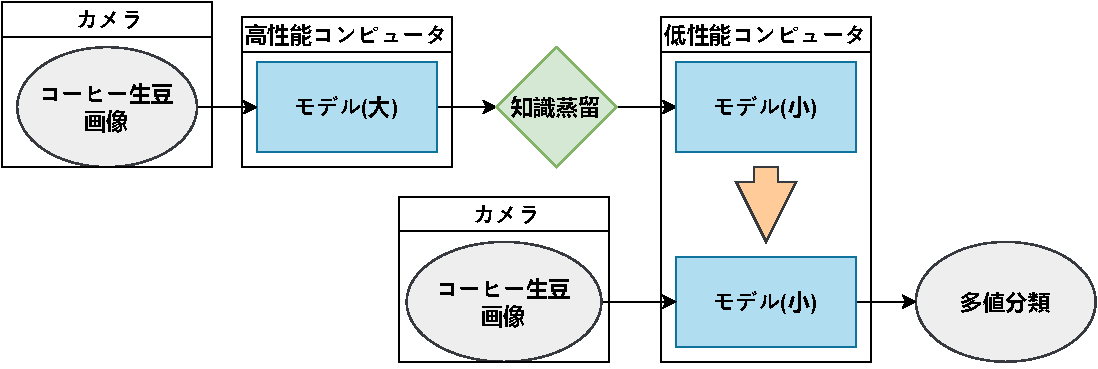
\includegraphics{system.pdf}}
    \caption{本研究のシステム構成図}
    \label{img:system} 
  \end{figurehere}

\section{データセットについて}
データセットは, 本研究で独自に収集したコーヒー生豆画像から構築した. 
まず, 人手によってラベル付けした良豆1,000 枚と, 欠け・奇形・カビなど確実に欠点豆と判断できる欠陥豆1,000枚を取得し, 合計2,000枚の元画像を用意した. 
画像サイズは224x224ピクセルに統一し, タスクは良豆と欠点豆の2値分類とした. 
また, モデルの汎化性能を高めるため, これらの元画像に対して40度ごとの回転および上下左右の反転によるデータ拡張を行った. 
その結果, 良豆・欠陥豆それぞれ36,000枚, 合計72,000枚からなるデータセットを構築した. 
本データセットを用いて教師モデルのベースライン評価および生徒モデルの学習・知識蒸留を行った. 

\section{結果と考察}
まず, 教師候補モデルとして, CNNベースからEfficientNet-B0, ResNet-50, TransformerベースからDeiT-Small, Swin-Smallを比較した. 
その結果, ResNet-50はAccuracy0.981, Recall0.990, F1-score 0.981, Swin-SmallはAccuracy 0.980, Recall 0.984, F1-score 0.980を達成し, いずれも高い性能を示した. 
特にRecallを重視した観点から, 欠点豆の見逃しを抑えつつ高いF1-scoreを維持できるResNet-50とSwin-Smallを教師モデルとして採用した. 

次に, これらの教師モデルから軽量CNN生徒モデルへの知識蒸留を行い, 生徒モデル単体との性能比較を行った. 
生徒モデル単体はAccuracy 0.928, Recall 0.910, F1-score 0.927と, 2値分類タスクとしてはすでに高い性能を示していた. 
ResNet-50を教師とした場合, 知識蒸留後の生徒モデルはAccuracy 0.907, Recall 0.885, F1-score 0.905となり, 生徒モデル単体よりも性能が低下した. 
一方, Swin-Smallを教師とした場合, 知識蒸留後の生徒モデルは Accuracy 0.945, Recall 0.943, F1-score 0.945 を達成し, Accuracy・Recall・F1-scoreの全てにおいて生徒モデル単体を上回る性能を示した. 
この結果から, 本研究ではTransformerベースのSwin-Smallを教師とすることで, 知識蒸留によって軽量生徒モデルが元の生徒モデルを越える性能を達成できた. 
これは, 教師モデルのアーキテクチャ選択が知識蒸留の効果に大きく影響することを示唆している. 

さらに, エッジデバイス上での実用度の評価を行った.

\section{終わりに}
本研究では, コーヒー生豆の欠点豆検出を対象として, 深層学習と知識蒸留を組み合わせたエッジデバイス向け欠陥検出システムの構築を行った. 
その結果, 独自に構築したデータセットに対して高い分類性能を示すことができた.  

{\small
\bibliography{bio. bib} %hoge. bibの名前
\bibliographystyle{unsrt}
}

\end{multicols}
\end{document}
